\documentclass[prb,preprint]{revtex4-1} 

\usepackage{amsmath}  
\usepackage{amsfonts} 
\usepackage{graphicx} 

\begin{document}


\title{Franck-Hertz Experiment; Measuring Energy Levels of Neon and Mercury}

\author{Jiajun Shi}
\email{jshi15@amherst.edu} 
\affiliation{Department of Physics, Amherst College, Amherst, MA, 01002}


\author{Danika Luntz-Martin}
\email{dluntzma@smith.edu}
\affiliation{Department of Physics, Smith College, Northampton, MA , 01063}


\date{\today}

\begin{abstract}


\end{abstract}


\maketitle 


\section{Introduction} 


\section{Methods}

\subsection{Neon}
\subsection{Mercury}


\section{Results}

\subsection{Neon}

We did four data runs using neon. For each run we recorded the accelerating voltage (x data) and the electron current measured by the anode, this current was recorded as a voltage measured across an internal resister. Each of our runs showed three discernible minima in the voltage corresponding to electron current, see the sample data run Figure~\ref{neon_data}. These dips are the voltages just before the electrons have enough energy (from the accelerating voltage) to reach the anode even after an inelastic collision with a neon atom. The apparent double minima, see the second and third dips in Figure~\ref{neon_data}, is most likely caused by by energy levels with very similar excitation energies.~\cite{newfeatures} Also of interest is the voltage corresponding to the steepest negative slope which is when the majority of electrons have enough energy to cite the neon atoms. However the location of the steepest negative slope was difficult to determine from our data, again see Figure~\ref{neon_data}.

\begin{figure}[h!]
\centering

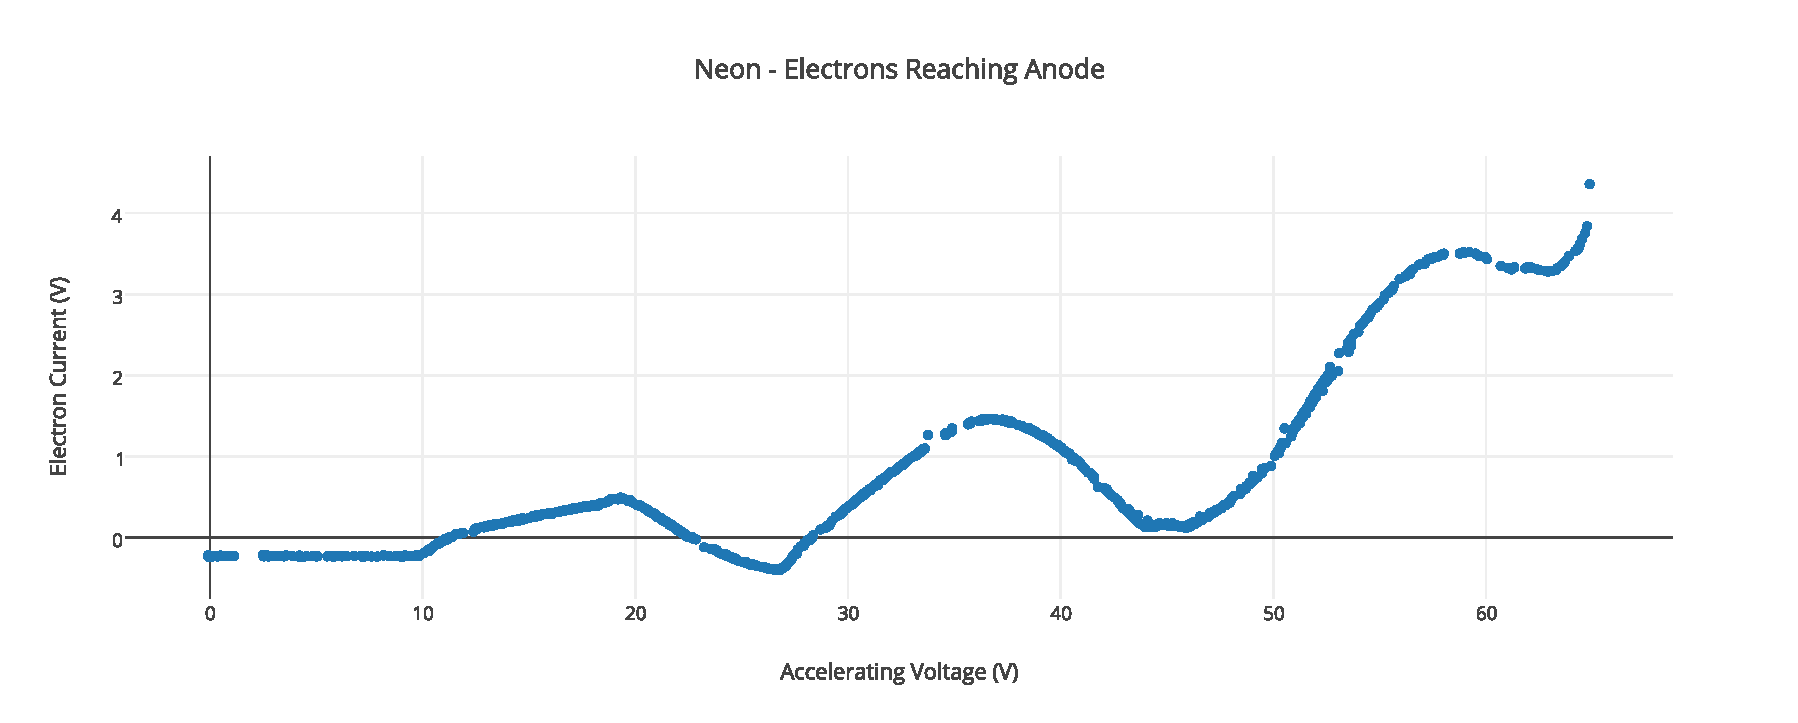
\includegraphics[width=6in]{neon_data.pdf}
\caption{Neon data with electron current as a voltage plotted against accelerating voltage. The three minima correspond to electrons exciting three neon atoms before reaching the anode. The double minima in the second and third dips is due to multiple excitations with similar energies.}

\label{neon_data}
\end{figure}


\subsection{Mercury}

Since the number of discernible dips for mercury depends on temperature, we collected data for 10$^{\circ}$C increments starting at 150$^{\circ}$C and ranging to 210$^{\circ}$C. From this data, see Figure~\ref{hg_data}, it can be seen that there is an optimum temperature at around 200$^{\circ}$C at which the most minima can be observed. 

\begin{figure}[h!]
\centering

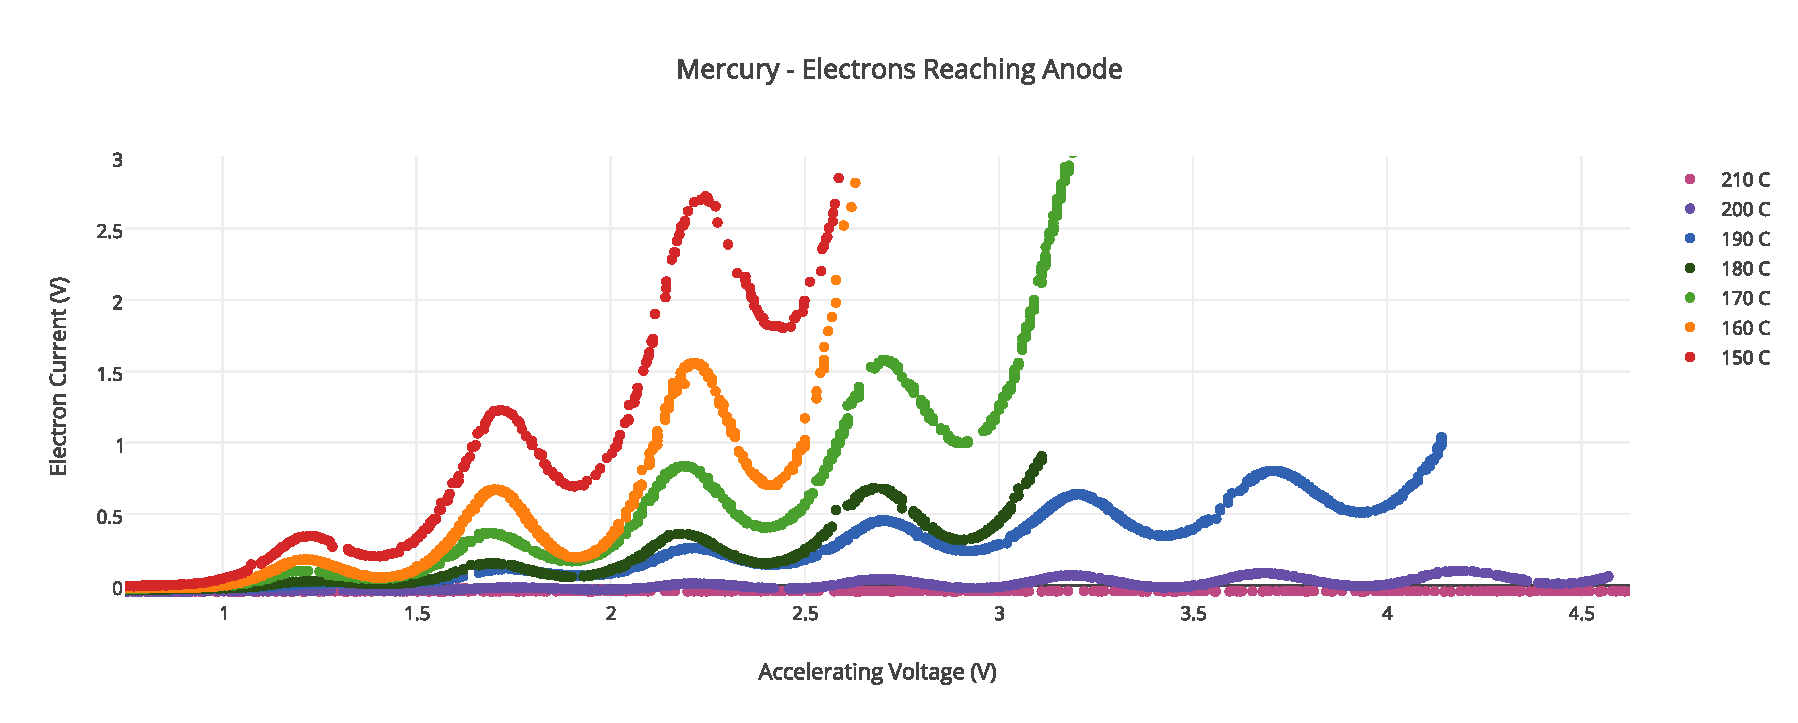
\includegraphics[width=6in]{hg_data.pdf}
\caption{Mercury data for temperatures ranging from 150$^{\circ}$C to 210$^{\circ}$C. The range of temperatures shows the optimum temperature to be approximately 190 - 200$^{\circ}$C. For higher temperatures, such as 210$^{\circ}$C, the minima in electron current are not discernible. For lower temperatures, for example 150$^{\circ}$C and 160$^{\circ}$C, there were fewer minima before the mercury atoms ionized.}

\label{hg_data}
\end{figure}

Using the information that we obtained about the optimum range of temperature, we took a more data using a lock-in. With the lock-in we took data from 185$^{\circ}$C to 215$^{\circ}$C in increments of 5$^{\circ}$C. The output from the lock-in, see Figure~\ref{hg_lockin}, is the derivative of the output without the lock-in. Therefore, the minima in the lock-in output correspond to the steepest negative slope of the direct output and the places the lock-in data passes through zero correspond to the minima and maxima of the direct output. The lock-in detector was highly sensitive to ionization of the mercury atoms. Our 185$^{\circ}$C data already showed significant reduction in the number of minima because of ionization. Because of space considerations we are not showing all of our lock-in data. Figure~\ref{hg_lockin} is the data collected for 205$^{\circ}$C and is a representative sample of the data collected.

\begin{figure}[h!]
\centering

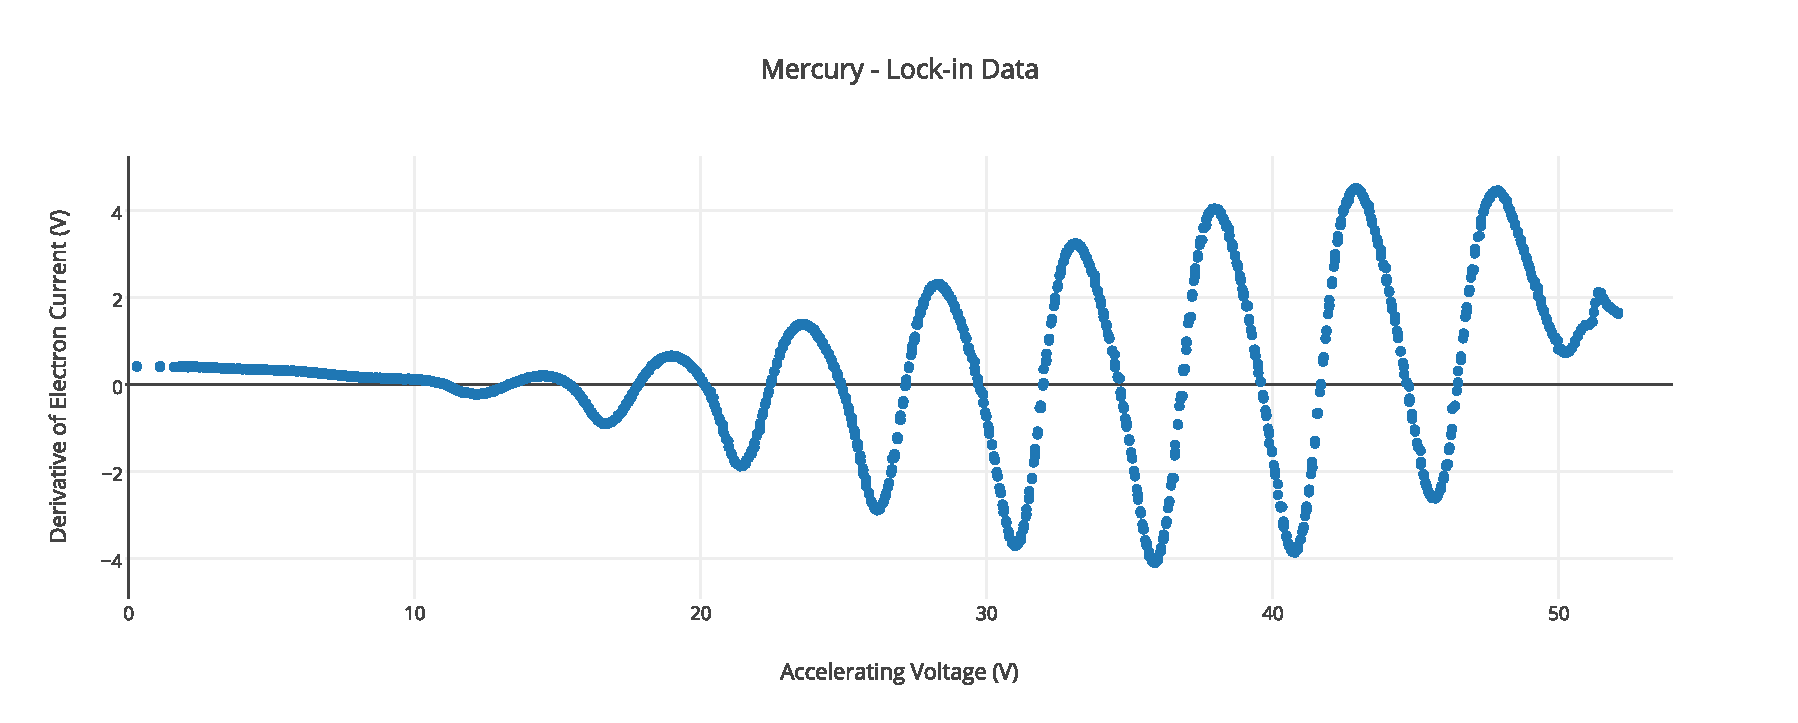
\includegraphics[width=6in]{hg_lockin.pdf}
\caption{Sample mercury data using lock-in detector at 205$^{\circ}$C. The lock-in output is the derivative of the direct output in Figure~\ref{hg_data}. Minima in the voltage correspond to the steepest negative slope of the electron current and the lock-in x intercepts with positive slopes correspond to the minima in the direct output.}

\label{hg_lockin}
\end{figure}



\section{Analysis}

\subsection{Neon}

To determine the energy needed to excite the neon atoms we needed to find the spacing of the minima in electron current (which we measured as a voltage.) We visually determined the locations of the minima and the steepest negative slopes with uncertainty for each of our data runs, see sample data in Figure~\ref{neon_data}. We then calculated the change in voltage between adjacent minima and between adjacent steepest slopes. These values can be seen in Table~\ref{neon_dvs}.

\begin{table}[h!]
\centering
\caption{ }
\begin{ruledtabular}
\begin{tabular}{c c c c}
$\Delta$V Minima & Error $\Delta$V Minima & $\Delta$V Steepest Slope &  Error $\Delta$V Steepest Slope\\
\hline	% horizontal line to separate headings from data
19.0 & 2.0 & 19.2 & 1.5  \\
16.4 & 2.0 & 19.5 & 1.5  \\
18.5 & 1.3 & 20.0 & 2.5  \\
17.6 & 1.6 & 18.5 & 2.5  \\
18.4 & 1.2 & 19.5 & 2.0  \\
17.0 & 1.5 & 18.8 & 2.0  \\
18.5 & 1.5 & 18.5 & 2.5  \\
17.5 & 2.5 & 19.5 & 2.0  \\

\end{tabular}
\end{ruledtabular}
\label{neon_dvs}
\end{table}

We then averaged these values and got 17.9 $\pm$ .3 eV as the average difference between the minima where the uncertainty is the standard deviation of the mean. From the difference between the steepest slopes we got an average value of 19.19 $\pm$ .19 eV. If we then average these two values, we get a final value of 18.5 $\pm$ .4 eV where uncertainty is again the standard deviation of the mean. This value agrees with our expectations because neon has a large number of transitions with energies ranging from 18.3 eV to 18.9 eV.

\subsection{Mercury}

Because the shape of our mercury data was highly dependent on temperature, the process by which we found the energy level was more involved. We began our analysis in a similar way to our analysis of neon by visually determining the location of the minima and steepest negative slope. However, when we calculated the difference in voltage between minima this method gave us an uncertainty on the order of 10$\%$. We then plotted the distance between minima versus the minima number as suggested by Rapior, Sengstock and Baev~\cite{newfeatures} and fit linear lines to the data for each temperature. Rapior, Sengstock and Baev found that the fit lines from each temperature converged toward the minima number .5. We found that the fit lines to our data did not converge at dip number .5, see Figure~|ref{hg_direct_plot}, furthermore the uncertainty for our minima was large enough to make our results imprecise and unsatisfying.

To improve our results, we used that data collected using the lock-in detector. Because the lock-in output is the derivative of the direct output it is the x intercept with a positive slope that corresponds to the minima in the direct data and the minima of the lock-in output corresponds to the steepest negative slopes of the direct output. The data with the least uncertainty was that data from the lock-in using the positve x intercepts to calculate the differences in voltage. From this data we found the values seen in Table~\ref{hg_lockin_table}.

\begin{table}[h!]
\centering

\caption{The difference in voltage for consecutive positive slope x intercepts in the electron current from the lock-in output. The first dip was indiscernible for the 215$^{\circ}$C data and the higher minima of the 195$^{\circ}$C and 185$^{\circ}$C data were lost due to ionization. The error for these values is ~1.3$\%$}

\begin{ruledtabular}
\begin{tabular}{c c c c c c c c}
Dips & $\Delta$V 215$^{\circ}$C & $\Delta$V 210$^{\circ}$C  & $\Delta$V 205$^{\circ}$C &$\Delta$V 200$^{\circ}$C  & $\Delta$V 195$^{\circ}$C  & $\Delta$V 195$^{\circ}$C &$\Delta$V 185$^{\circ}$C  \\
\hline	% horizontal line to separate headings from data
1 - 2 &         & 4.67 & 4.53 & 4.42 & 4.36 & 4.58 & 4.51 \\
2 - 3 & 4.63 & 4.57 & 4.63 & 4.61 & 4.63 & 4.78 & 4.82 \\
3 - 4 & 4.67 & 4.69 & 4.63 & 4.73 & 4.84 & 4.87 & 4.90 \\
4 - 5 & 4.74 & 4.79 & 4.89 & 4.83 & 4.87 & 4.93 &         \\
5 - 6 & 4.76 & 4.80 & 4.87 & 4.88 & 4.95 & 4.99 &         \\
6 - 7 & 4.76 & 4.82 & 4.84 & 4.91 &         & 5.05 &         \\
7 -8  & 4.76 & 4.73 & 4.77 & 4.85 &         & 4.90 &         \\

\end{tabular}
\end{ruledtabular}
\label{hg_lockin_table}
\end{table}

The results of Table~\ref{hg_lockin_table} are plotted in Figure~\ref{lockin_intercepts}. 

\begin{figure}[h!]
\centering

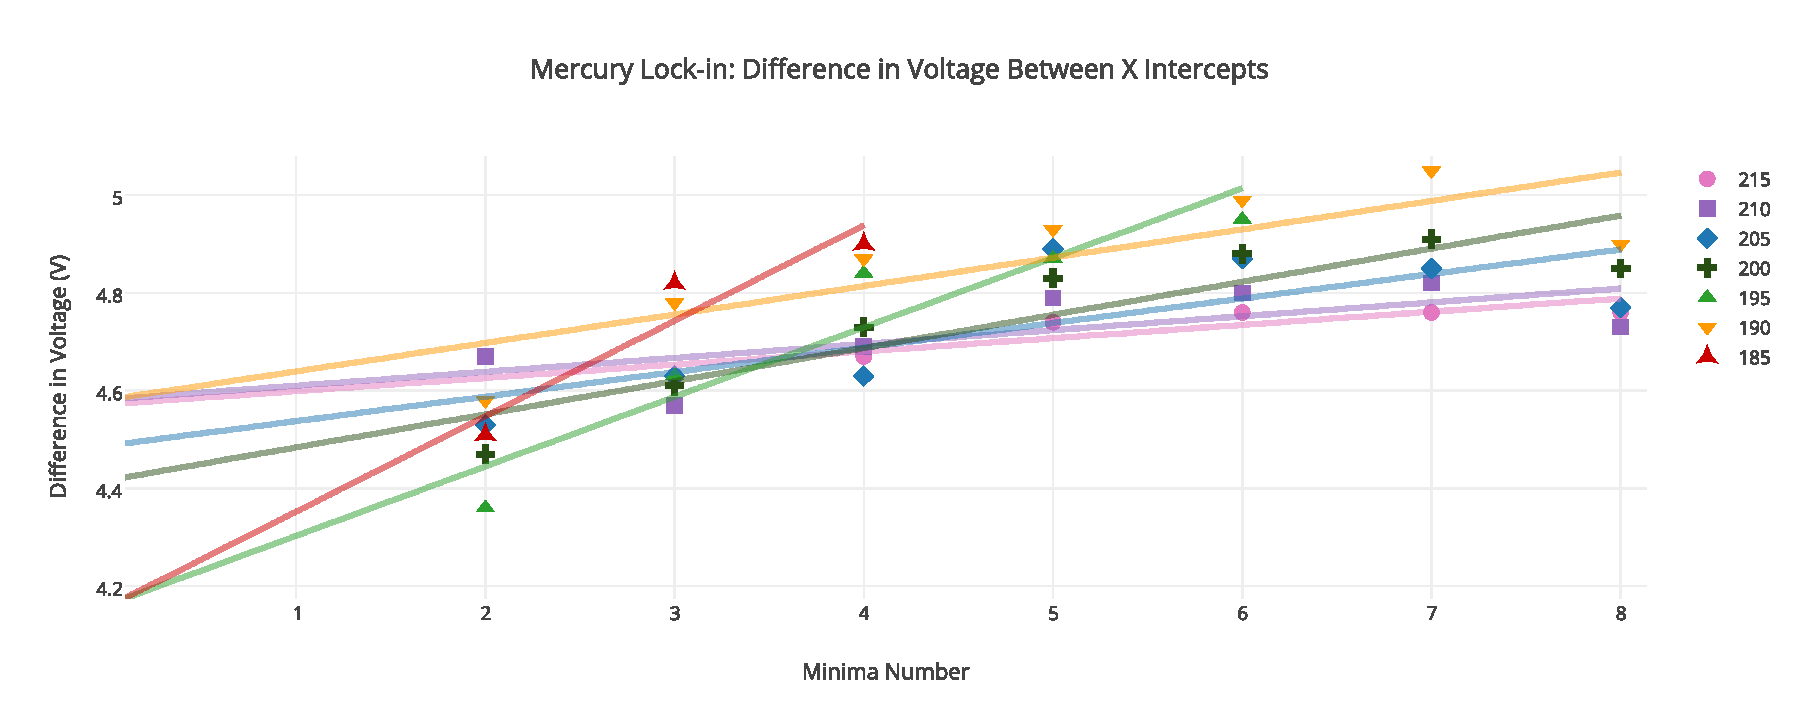
\includegraphics[width=6in]{lockin_intercepts.pdf}
\caption{The plot of the difference in voltage between minima versus the number of the minimum. All values have an uncertainty of ~1.3$\%$. The lines are linear fits to the data for each temperature. The two fits with steeper slopes correspond to the 195$^{\circ}$C and 185$^{\circ}$C data sets which were truncated due to ionization.}

Following the analysis outlined by Rapior, Sengstock and Baev, we used our fit lines to extrapolate to the voltages corresponding to a minima number of .5. Averaging these values gave us XXX $\pm$ XXX where the uncertainty is the standard deviation of the mean. The results obtained from all of our mercury data are in Table~\ref{hg_results}, not the much larger uncertainties for the direct output data and lock-in data were we locked at the minima.  

\label{lockin_intercepts}
\end{figure}



\section{Discussion}


\section{Conclusion}



\begin{thebibliography}{9}


\bibitem{newfeatures} Gerald Rapior, Klaus Sengstock, and Valery Baev, "New Features of the Franck-Hertz Experiment,"  Am. J. Phys. \textbf{74}, 423--428 (2006). 

\bibitem{melissanos} Adrian C. Melissanos and Jim Napoitano, \textit{Experiments in Modern Physics} 2nd edition (Academic Press, Boston, 2003).

\bibitem{hyperphysics} Hyper-Physics: Franck-Hertz Experiment Website \url{<http://hyperphysics.phy-astr.gsu.edu/hbase/frhz.html>}

\end{thebibliography}


\end{document}
